\documentclass[tikz,border=6pt]{standalone}
\usetikzlibrary{arrows.meta,positioning,calc,fit,backgrounds}
\newcommand{\NodeW}{30mm}
\definecolor{ink}{HTML}{1A1A1A}
\definecolor{rule}{HTML}{9AA3AB}
\definecolor{edge}{HTML}{555555}
\definecolor{tint}{HTML}{F7E9E9}
\definecolor{faint}{HTML}{C8CFD5}
\begin{document}
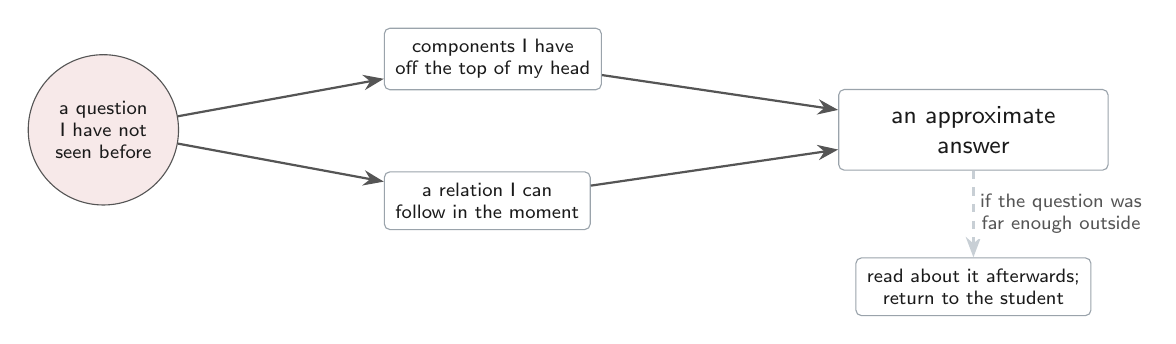
\begin{tikzpicture}[
  font=\sffamily\small,
  kc/.style={draw=rule, fill=white, rounded corners=2pt, text width=\NodeW,
             align=center, inner sep=6pt, text=ink},
  small/.style={draw=rule, fill=white, rounded corners=2pt, align=center,
                inner sep=4pt, text=ink, font=\sffamily\scriptsize},
  src/.style={draw=edge, fill=tint, circle, inner sep=5pt, text=ink,
              font=\sffamily\scriptsize, align=center},
  rel/.style={-{Stealth[length=2.6mm]}, draw=edge, thick},
  weak/.style={-{Stealth[length=2.6mm]}, draw=faint, thick, dashed},
  lab/.style={font=\sffamily\scriptsize, text=edge, align=center,
              fill=white, inner sep=2pt}
]
\node[src] (q) {a question\\I have not\\seen before};
\node[small, right=26mm of q, yshift=9mm] (a) {components I have\\off the top of my head};
\node[small, right=26mm of q, yshift=-9mm] (b) {a relation I can\\follow in the moment};
\node[kc, right=30mm of a, yshift=-9mm] (ans) {an approximate\\answer};
\node[small, below=11mm of ans] (later) {read about it afterwards;\\return to the student};
\draw[rel] (q) -- (a);
\draw[rel] (q) -- (b);
\draw[rel] (a) -- (ans);
\draw[rel] (b) -- (ans);
\draw[weak] (ans) -- node[lab,midway,right]{if the question was\\far enough outside} (later);
\end{tikzpicture}
\end{document}
